\begin{ex}
Um paraquedista programou seu pouso em uma fazenda retangular que possui um lago circular em seu interior, conforme indicado na figura. Se as condições climáticas não favorecem o paraquedista , o local de pouso pode se tornar aleatório. Qual é, nesse caso, a probabilidade de o paraquedista pousar em terra?\\
Adote $\pi = 3$
\begin{center}
    
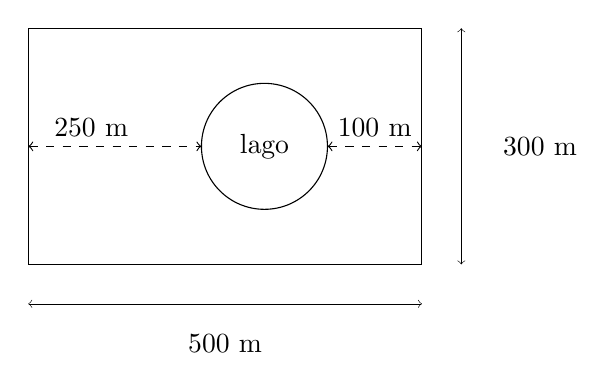
\begin{tikzpicture}
  \draw (0,0)--(5,0)--(5,3)--(0,3)--(0,0);    
  \draw (3,1.5) circle [radius = .8];
  \draw [<->] [dashed] (0,1.5)--(2.2,1.5);
  \draw node [above] at (.8,1.5) {250 m};
  \draw node [above] at (4.4,1.5) {100 m};
  \draw [<->] [dashed] (3.8,1.5)--(5,1.5);
  \draw node at (3,1.5) {lago};
  \draw [<->] [very thin] (0,-.5)--(5,-.5);
  \draw node at (2.5,-1) {500 m};
  \draw  [<->] [very thin] (5.5,0)--(5.5,3);
  \draw node at (6.5,1.5) {300 m};

\end{tikzpicture}
\end{center}
  \begin{sol}
    \phantom{A} \\
    A(terra) = $(500\cdot300) - 3\cdot(75)^2= 133125  m^2 \Longrightarrow p=\frac{133125}{150000}=88,75\%$ 
  \end{sol}
\end{ex}